\documentclass[presentation]{subfiles}
\onlyinsubfile{}
\setbeamersize{description width=30mm}
\begin{document}
\begin{frame}<-3>[label=returnable]{\only<-3>{Before We Get Started\dots}\only<4->{Old Wine in New Bottles}}
      \begin{description}
        \item<1-> [Crowd work] Digitally mediated \alert{information work}
        (e.g. Amazon Mechanical Turk, UpWork)\\
          \scriptsize{\textcite{crowdworkFuture}}\normalsize{}
        \item<2-> [Gig work] Digitally mediated (often \alert{physically embodied}) one--off jobs,
        such as
        \emph{driving for hire},
        \emph{courier services},
        and \emph{administrative support}\\
          \scriptsize{\textcite{friedman2014workers,Parigi:2016:GE:3026779.3013496}}\normalsize{}
        \item<3-> [On--demand~work] Crowd work and gig work, collectively
        \item<5-> [Piecework] Payment for \emph{output} rather than for \emph{time}
      \end{description}
\end{frame}


\begin{frame}[standout]
On--demand work is a modern instantiation of a much older phenomenon
--- \alert{piecework}.

{\normalsize The historical arc of piecework
can shed light on persistent questions
in this ongoing phenomenon of on--demand work.}
\end{frame}

\againframe<4->{returnable}

\begin{frame}[t]{What is piecework?}
\centering
  \emph{Payment for \textbf{output} rather than for \textbf{time}}
\vspace*{2mm}
\begin{columns}
  \begin{column}{0.33\textwidth}
    \centering
    Textiles
    \begin{figure}
    \begin{overlayarea}{\textwidth}{33mm}
    \begin{minipage}[c][33mm]{\textwidth}
      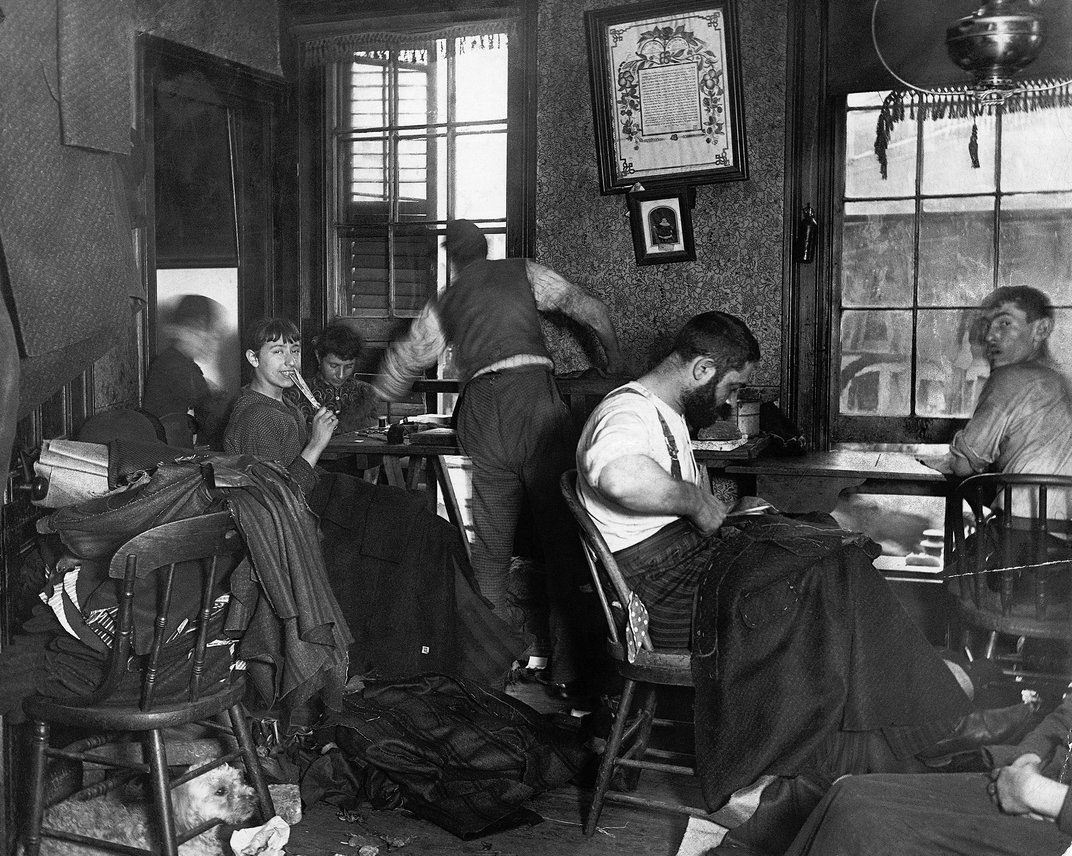
\includegraphics[width=\textwidth]{figures/pieceworkers.jpg}
    \end{minipage}
    \end{overlayarea}
    \end{figure}
  \end{column}
  \begin{column}{0.33\textwidth}
    \centering
    Automobiles
    \begin{figure}
    \begin{overlayarea}{\textwidth}{33mm}
    \begin{minipage}[c][33mm]{\textwidth}
      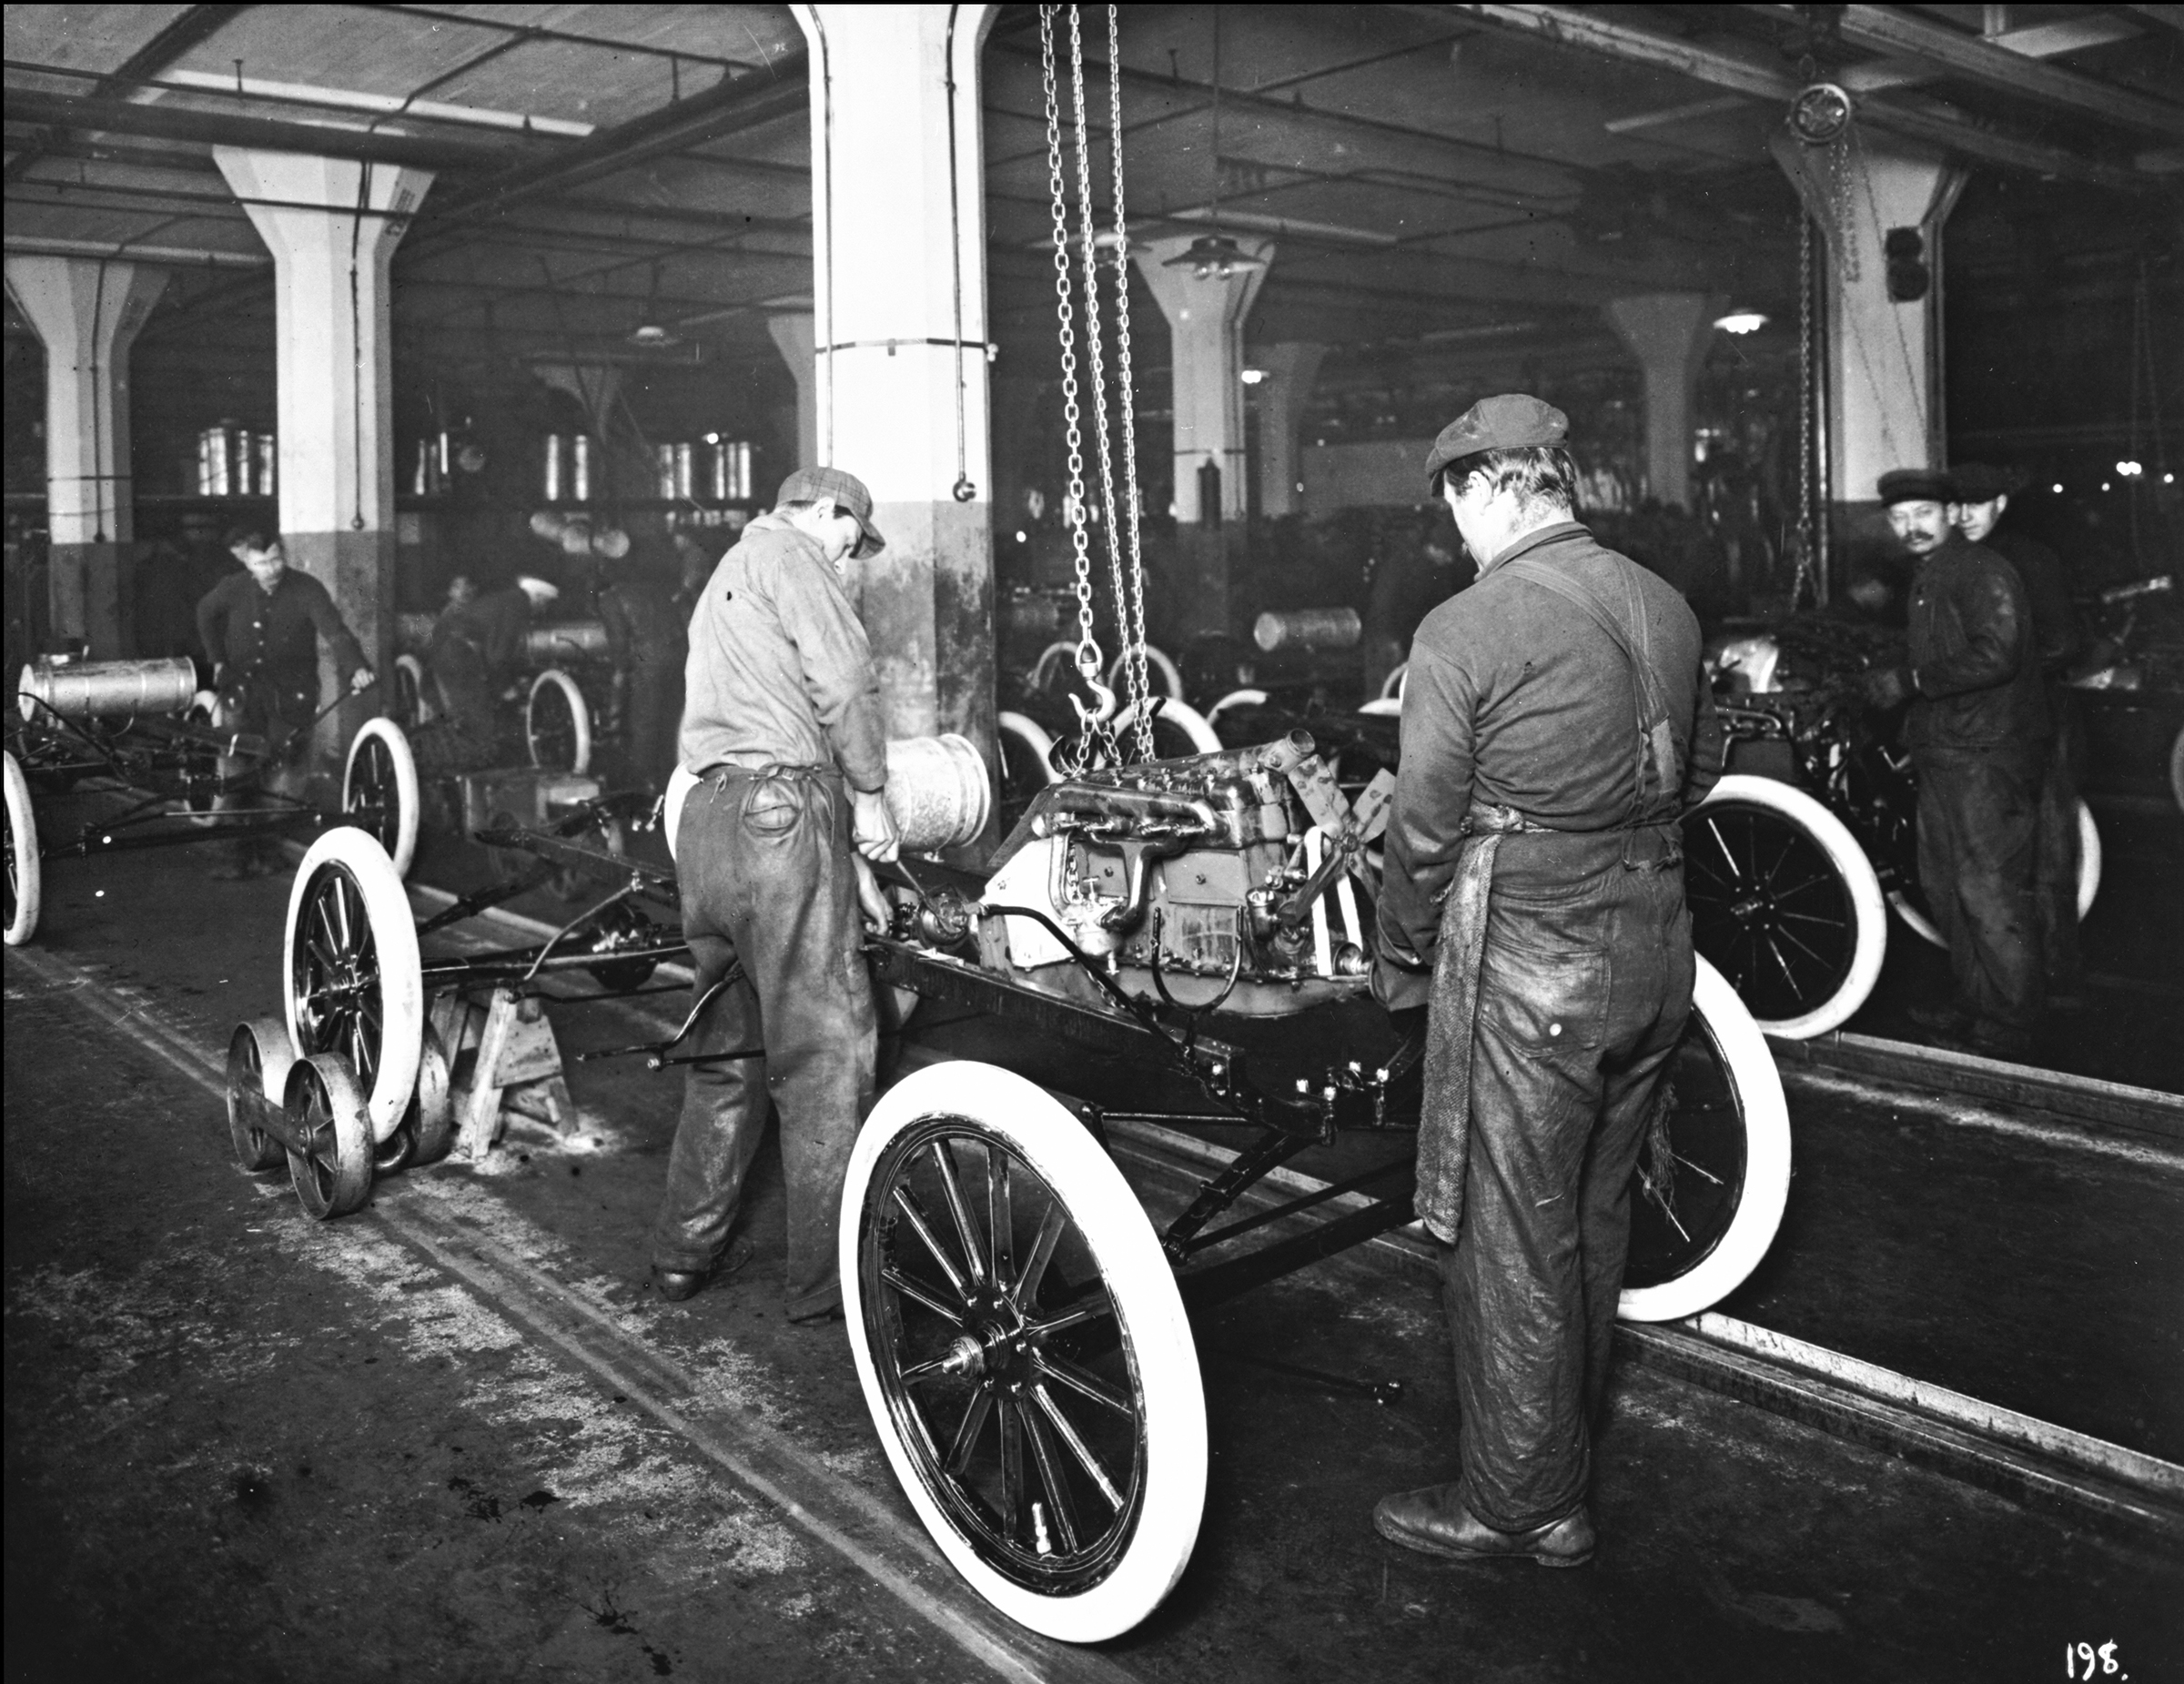
\includegraphics[width=\textwidth]{figures/photo/ford_assembly_line.jpg}
    \end{minipage}
    \end{overlayarea}
    \end{figure}
  \end{column}
  \begin{column}{0.33\textwidth}
    \centering
    Metalwork
    \begin{figure}
    \begin{overlayarea}{\textwidth}{33mm}
    \begin{minipage}[c][33mm]{\textwidth}
      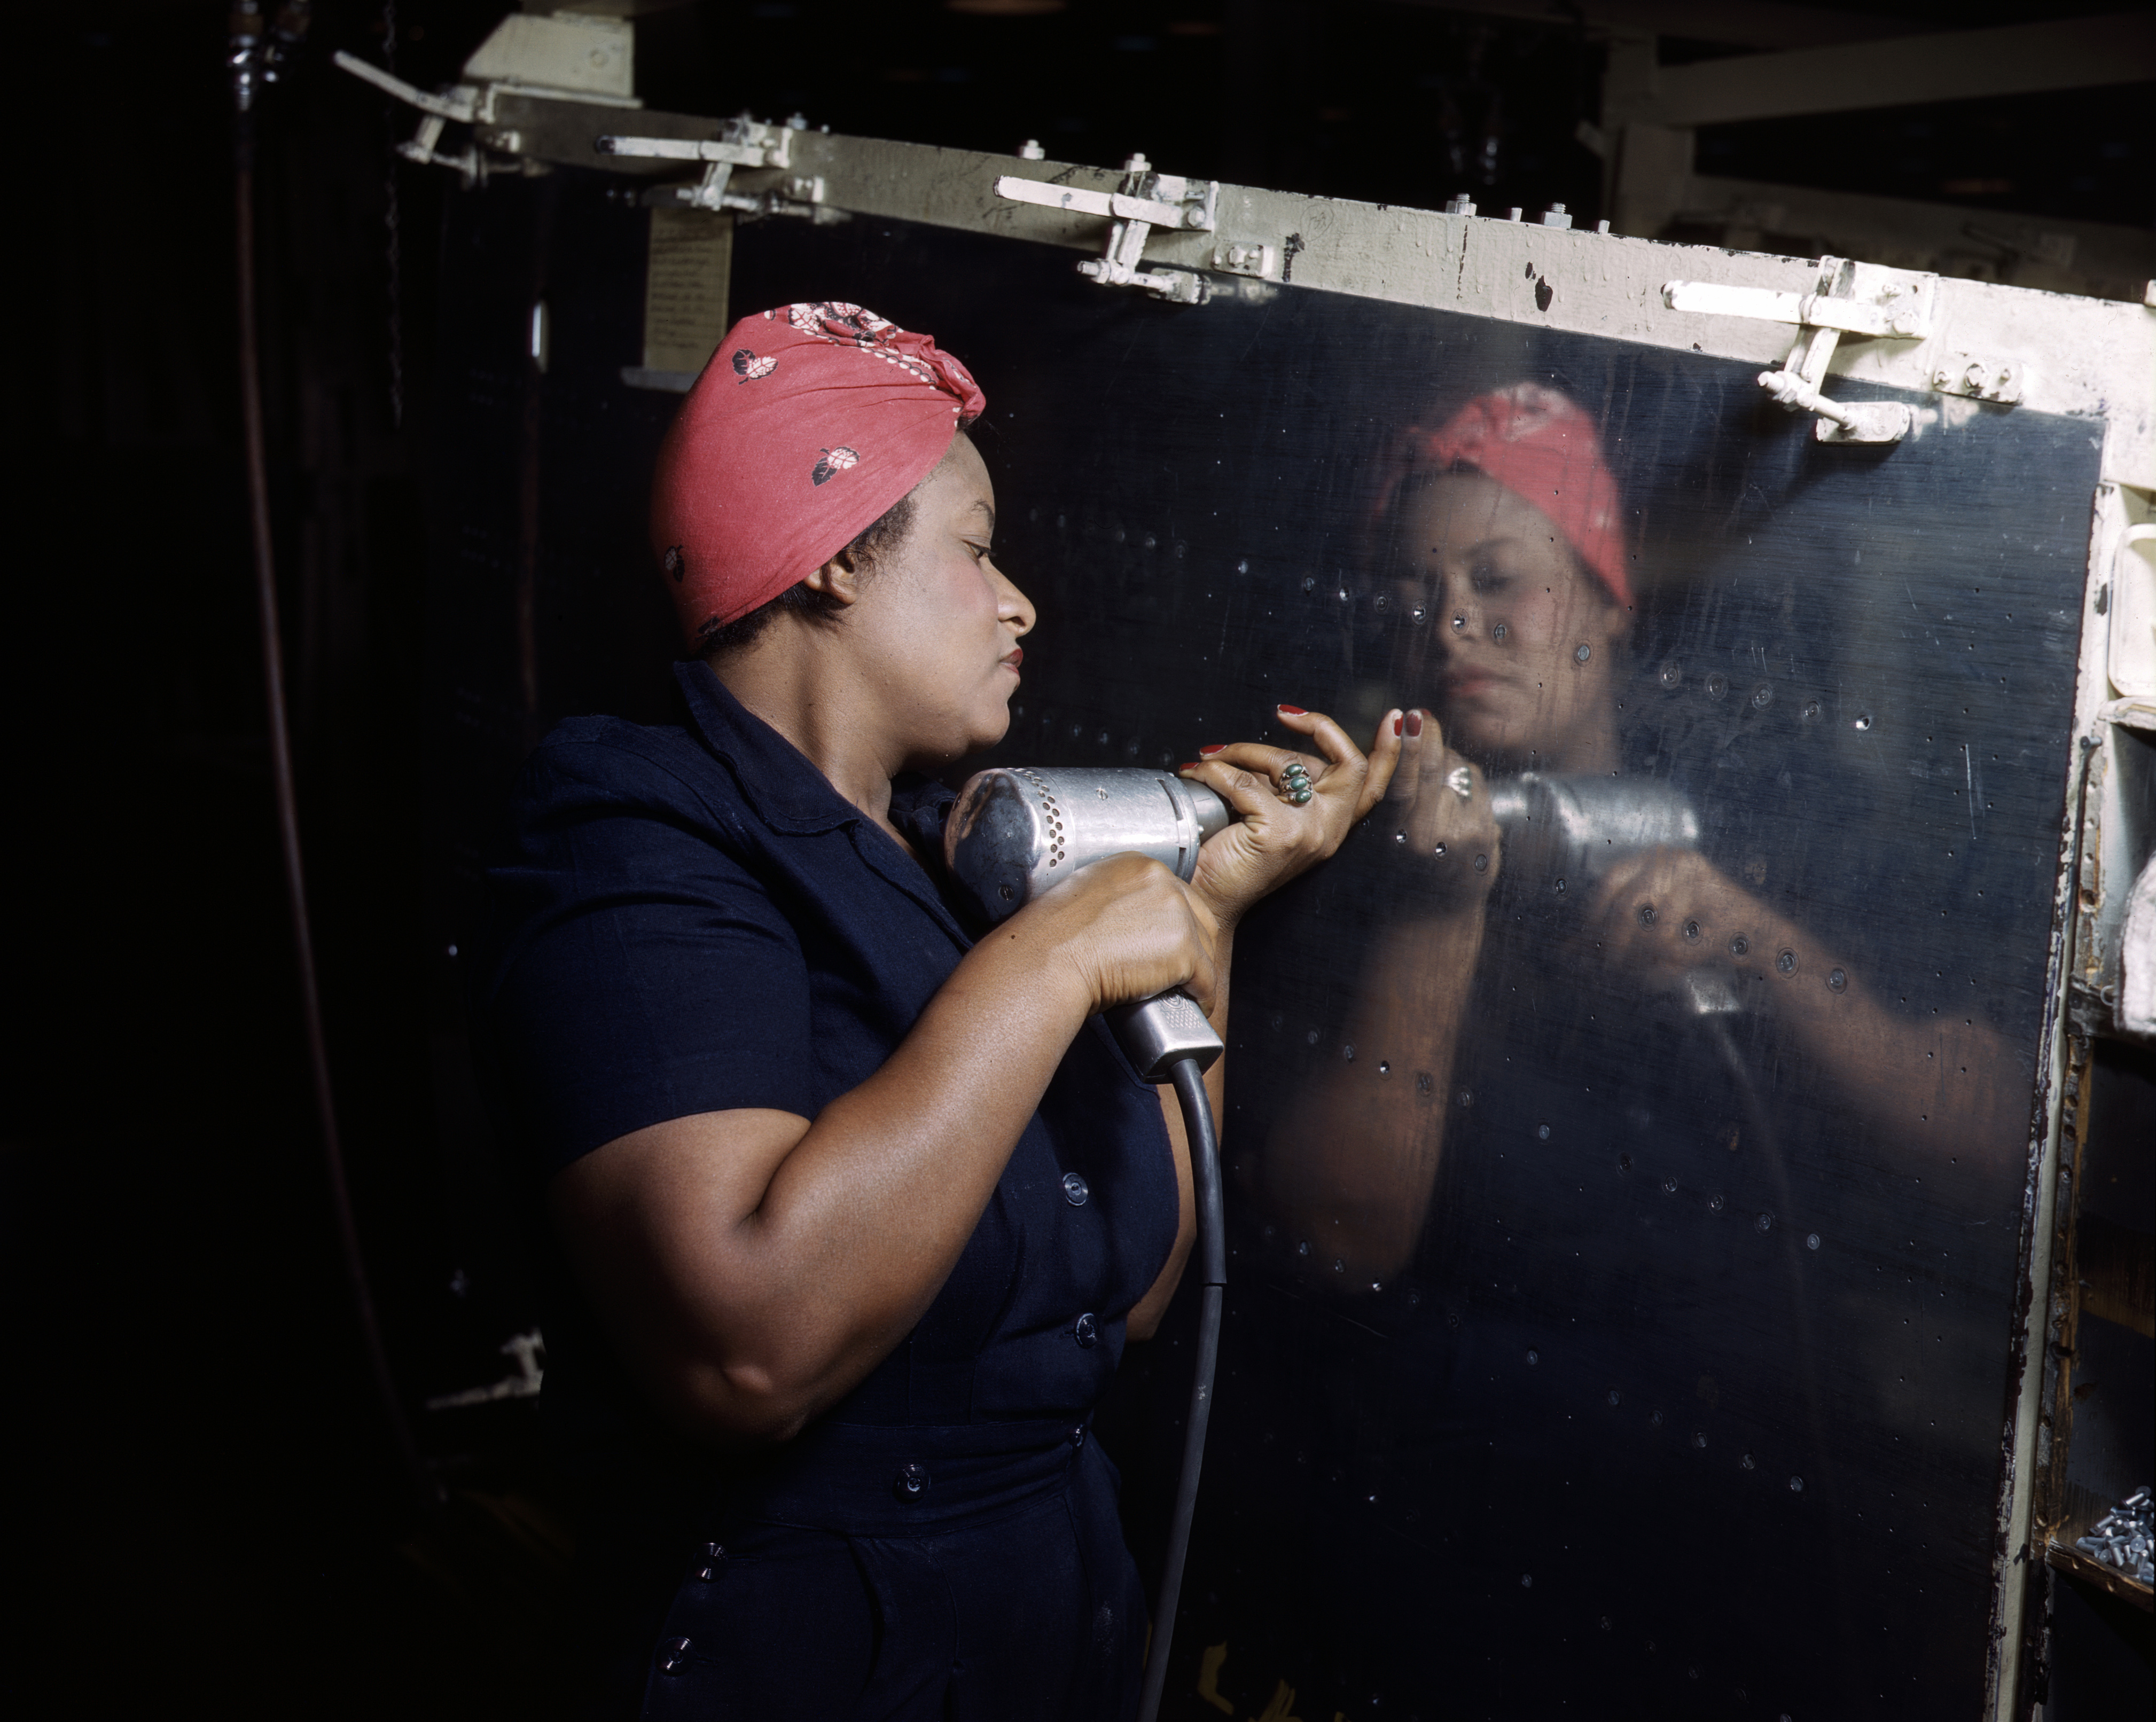
\includegraphics[width=\textwidth]{figures/photo/Rosie_the_Riveter_(Vultee)_DS.jpg}
    \end{minipage}
    \end{overlayarea}
    \end{figure}
  \end{column}
\end{columns}

\visible<2->{
  \begin{columns}
  \centering
    \begin{column}{0.33\textwidth}
    \centering
      Crowd work
    \begin{figure}
      \begin{overlayarea}{\textwidth}{15mm}
      \begin{minipage}[c][15mm]{\textwidth}
        
\includegraphics[width=\textwidth]{figures/amt.png}
      \end{minipage}
      \end{overlayarea}
    \end{figure}
    \end{column}
    \begin{column}{0.33\textwidth}
    \centering
      Gig Work
    \begin{figure}
    \begin{overlayarea}{\textwidth}{15mm}
      \begin{minipage}[c][15mm]{\textwidth}
        
\includegraphics[width=\textwidth]{figures/uber.png}
      \end{minipage}
      \end{overlayarea}
    \end{figure}
    \end{column}
  \end{columns}
}

\end{frame}


% \begin{frame}{Why Piecework?}
% What makes on--demand work another instantiation of piecework?

% \ali{piecework }
% \end{frame}


\begin{frame}[standout]
    What will be the future of work?
\end{frame}

\begin{frame}{What will be the future of work?}
    How will \alert{technology} affect the complexity of the work that on--demand workers do?

    What are the \alert{limits} of complexity in on--demand work?
\end{frame}


\begin{frame}{Thesis}
    This question --- and others like it --- has been asked before.

    History can help us answer them today.

    We'll reach into the history of \alert{piecework}
    --- of human computers, match stick makers, and metalworkers ---
    and show how the \alert{history} of their work can
    inform answers to questions about the \alert{future} of digital work.
\end{frame}


\notinsubfile{
  \subfile{timeline.tex}
}


\begin{frame}{Introduction}
  We hope to provide:
      \begin{itemize}
        \item A useful ontological lens for making sense of on--demand work as a resurgence of \alert{piecework}
        \item A method for making sense of contemporary phenomena through \alert{historical analysis}
      \end{itemize}
\end{frame}


\begin{frame}{Comparative Historical Analysis}
\begin{itemize}
  \item Historical analysis isn't new
  \begin{itemize}
    \item In general\\
    \scriptsize{\textcite{rosenberg1994exploring,rosenberg1982inside}}\normalsize{}
    \item In HCI\\
    \scriptsize{\textcite{Wyche2006,bodker1993historical}}\normalsize{}
  \end{itemize}
  \item Still, it's an underutilized method
  \begin{itemize}
    \item Provide some basic framing for \emph{ostensibly} new phenomena
    \item \emph{Explicate} our theoretical grounding
    \item Flesh out \emph{differences} and their implications
  \end{itemize}
\end{itemize}
\end{frame}



\onlyinsubfile{
  \printbibliography{}
}

\end{document}